% tags: arc edgeLabel label blockDiagram house background align
\PassOptionsToPackage{usenames,dvipsnames}{xcolor}
\documentclass[tikz, border=10pt]{standalone}

\usepackage{verbatim}
\usepackage{amsmath}

\tikzset{>=stealth}
\tikzstyle{every node}=[align=center]
\usetikzlibrary{spy,shadows,arrows,shapes,positioning,calc,backgrounds,fit,automata}

\begin{document}
\pgfdeclarelayer{bg}
\pgfdeclarelayer{fg}
\pgfsetlayers{bg,main,fg}
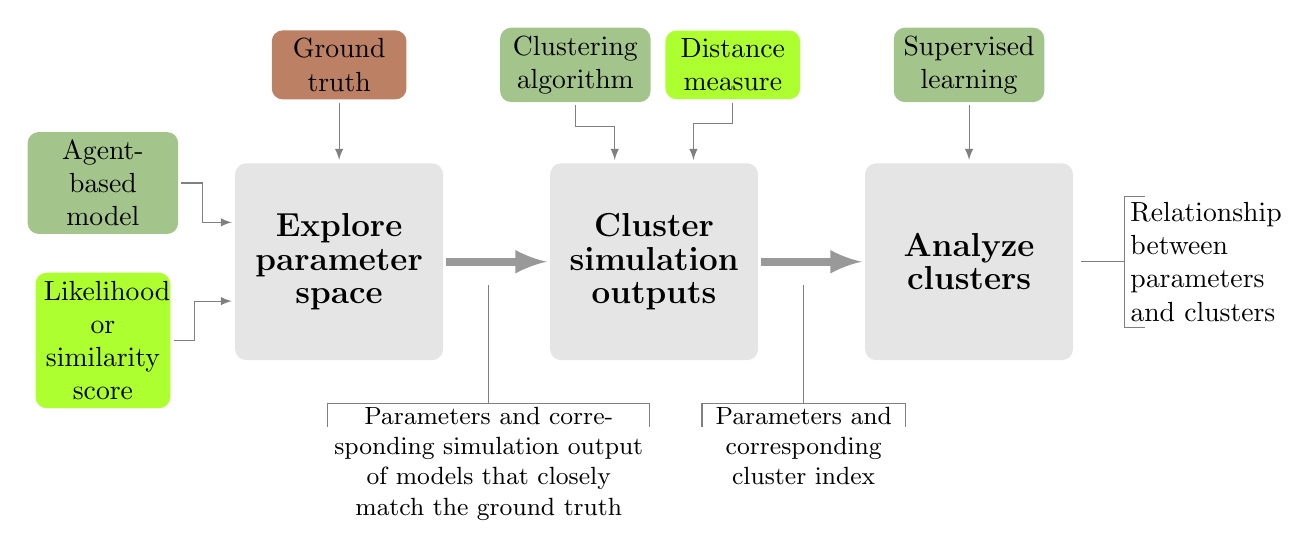
\begin{tikzpicture}
[blk/.style={inner sep=2pt,fill=black!10,rounded corners,text width=2.5cm,minimum height=2.5cm},
dat/.style={inner sep=3pt,fill=Sepia!40,rounded corners,text width=1.5cm},
desc/.style={inner sep=1pt,text width=4cm,font=\small},
alg/.style={inner sep=3pt,fill=OliveGreen!40,rounded corners,text width=1.7cm},
measure/.style={inner sep=3pt,fill=GreenYellow,rounded corners,text
width=1.5cm},
every node/.style={inner sep=5pt,align=center},
blkedge/.style={draw=black!40,>=latex, shorten >=1pt, shorten <=1pt, line
width=1mm},
datedge/.style={draw,>=latex, shorten >=1pt, shorten <=1pt,draw=black!50},
node distance=3cm]

%% grid
\node[blk] (explore) {\textbf{\large Explore\\ parameter space}};
\node[alg,left of=explore,shift={(0,1)}] (abm) {Agent-based model};
\draw[datedge,->] (abm.east) -- +(.3,0) |- ($(explore.west)+(0,.5)$);
\node[measure,left of=explore,shift={(0,-1)}] (score) {Likelihood or similarity score};
\draw[datedge,->] (score.east) -- +(.3,0) |- ($(explore.west)+(0,-.5)$);
\node[above of=explore,dat,shift={(0,-.5)}] (gt) {Ground truth};
\draw[datedge,->] (gt) -- (explore);
%%
\node[blk,right of=explore,shift={(1,0)}] (cluster) {\textbf{\large Cluster \\simulation outputs}};
\draw[blkedge,->] (explore) -- (cluster);
\node[alg,above of=cluster,shift={(-1,-.5)}] (xmeans) {Clustering algorithm};
\draw[datedge,->] (xmeans.south) -- +(0,-.3) -| ($(cluster.north)+(-.5,0)$);
\node[measure,above of=cluster,shift={(1,-.5)}] (dist) {Distance measure};
\draw[datedge,->] (dist.south) -- +(0,-.3) -| ($(cluster.north)+(.5,0)$);
%%
\node[blk,right of=cluster,shift={(1,0)}] (analyze) {\textbf{\large Analyze clusters}};
\draw[blkedge,->] (cluster) -- (analyze);
\node[alg,above of=analyze,shift={(0,-.5)}] (cart) {Supervised learning};
\draw[datedge,->] (cart) -- (analyze);
\node[anchor=west,text width=1.9cm,align=left,right of=analyze,inner sep=2pt] (rel) {Relationship between parameters and clusters};
\draw [datedge] ($(analyze.east)+(.1,0)$) -- (rel) -|
(rel.north west) -- +(.3,0);
\draw [datedge] (rel) -| (rel.south west) -- +(.3,0);
%% lower part
\node[desc,below of=explore,anchor=north,shift={(1.9,1.2)}] (fit)
{Parameters and corresponding simulation output of models that closely
match the ground truth};
\draw [datedge,shorten >=0pt,shorten <=0pt] (fit.north) -- +(0,1.5);
\draw [datedge,shorten >=0pt,shorten <=0pt] (fit.north) -| ($(fit.north west)+(0,-.3)$);
\draw [datedge,shorten >=0pt,shorten <=0pt] (fit.north) -| ($(fit.north east)+(0,-.3)$);
%%
\node[desc,text width=2.5cm,below of=cluster,anchor=north,shift={(1.9,1.2)}] (clustered)
{Parameters and corresponding cluster index};
\draw [datedge,shorten >=0pt,shorten <=0pt] (clustered.north) -- +(0,1.5);
\draw [datedge,shorten >=0pt,shorten <=0pt] (clustered.north) -| ($(clustered.north west)+(0,-.3)$);
\draw [datedge,shorten >=0pt,shorten <=0pt] (clustered.north) -| ($(clustered.north east)+(0,-.3)$);
\end{tikzpicture}
\end{document}
%% spatial
\node[blk,right of=grid] (spatial) {\textbf{\large Spatial \\ disaggregation of
production} \\ \smallskip Country/province production to cells};
\draw[datedge,<-] ($(spatial.north)+(-.5,0)$) |- +(-1cm,1cm) node[text
width=3cm,anchor=east] {Production volume (country or province)};
\draw[datedge,<-] ($(spatial.north)+(+.5,0)$) -- +(0cm,1.2cm) node[text
width=1.5cm,anchor=south] {MAPSPAM};
%% temporal
\node[blk,right of=spatial] (temporal) {\textbf{\large Temporal
    disaggregation} \\
\smallskip Annual/seasonal to monthly production};
\draw[blkedge,->] (spatial) -- (temporal);
\draw[datedge,<-] ($(temporal.north)+(-.75,0)$) |- +(-.4cm,.8cm)
node[anchor=east] {Temperature};
\draw[datedge,<-] ($(temporal.north)+(0,0)$) -- +(0cm,1cm)
node[anchor=south] {Seasonal production};
\draw[datedge,<-] ($(temporal.north)+(.75,0)$) |- +(.4cm,.8cm)
node[anchor=west] {Precipitation};
%% locality
\node[blk,below of=temporal,shift={(0,-.2)}] (locality) {\textbf{\large Locality
construction} \\\smallskip Parameters: radius and population threshold};
\draw[blkedge,->] (temporal) -- node [text width=3.4cm,anchor=west] {Monthly
cell level production indicating host presence} (locality);
\draw[datedge,<-] ($(locality.south)+(.5,0)$) |- +(.4cm,-.6cm)
node[text width=2cm,anchor=west] {Population (Landscan)};
\draw[datedge,<-] ($(locality.south)+(-.5,0)$) -- +(0cm,-.8cm)
node[text width=5cm,anchor=north] {Major consumption and production centers};
%% gravity
\node[blk,left of=locality,shift={(-2.6,0)}] (gravity) {\textbf{\large Monthly trade flows
}\\\smallskip Gravity model parameters $\beta$ and $\kappa$};
\draw[blkedge,->] (locality) -- (gravity) node[midway,text width=3.3cm,anchor=south]
{Production and population aggregated at locality level};
\draw[datedge,<-] ($(gravity.south)+(0,0)$) -- +(0cm,-.7cm)
node[text width=5cm,anchor=north] {Travel duration between localities (Google Maps)};
%% final
\draw[datedge,->] (gravity) -- +(-2.5,0) node[align=left,inner
sep=0,shift={(-.1,0)},anchor=east,text width=2.5cm]
{{Hierarchical spatio-temporal network of cells}};
%%
\begin{pgfonlayer}{bg}
\newcommand{\Red}{RedViolet!15}
\newcommand{\Blue}{TealBlue!15}
\newcommand{\DarkRed}{RedViolet!60}
\newcommand{\DarkBlue}{TealBlue!60}
\draw[fill=\Red,draw=none] ($(grid.north
west)+(-.1,.1)$) rectangle ($(temporal.south east)+(.1,-.1)$);
%% \draw[\Red,ultra thick] ($(temporal.north east)+(.1,.1)$) -- +(.4,0)
%% arc(90:-90:1.6) -- +(-.4,0);
%% \draw[\DarkRed,ultra thick] ($(temporal.east)+(.2,0)$) --
%% ($(temporal.north east)+(1,.1)$) node (anch) {} -- ++(1.3,0) -- ++(0,-3.2)
%% -- ($(anch)+(0,-3.2)$) -- cycle;
\draw[\DarkRed,ultra thick] ($(temporal.east)+(.2,0)$) --
($(temporal.north east)+(.7,-.1)$) node (anch) {} -- ++(.01,0) -- ++(0,-2.8)
-- ($(anch)+(0,-2.8)$) -- cycle;
%% \draw[\DarkRed,ultra thick] ($(temporal.east)+(.2,0)$) --
%% ($(temporal.north east)+(.7,-.2)$) -- ++(0,-2.6) -- cycle;
\draw[fill=\Blue,draw=none] ($(gravity.north
west)+(-.1,.1)$) rectangle ($(locality.south east)+(.1,-.1)$);
%% \draw[\DarkBlue,ultra thick] ($(locality.east)+(.2,0)$) --
%% ($(locality.north east)+(1,.1)$) node (anch) {} -- ++(1.3,0) -- ++(0,-3.2)
%% -- ($(anch)+(0,-3.2)$) -- cycle;
\draw[\DarkBlue,ultra thick] ($(locality.east)+(.2,0)$) --
($(locality.north east)+(.7,-.1)$) node (anch) {} -- ++(.01,0) -- ++(0,-2.8)
-- ($(anch)+(0,-2.8)$) -- cycle;
\end{pgfonlayer}
\node at (temporal.east) [inner sep=0cm,anchor=west,text
width=1.56cm,text =black,shift={(.8,0)},align=left] {\bfseries Self-mediated dispersal};
\node at (locality.east) [inner sep=0cm,anchor=west,text
width=1.56cm,shift={(.8,0)},align=left] {\bfseries Human-mediated dispersal};
\end{tikzpicture}
\end{document}
